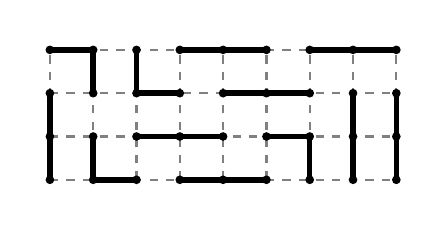
\begin{tikzpicture}[scale = 0.55]
  \draw[white] (0.5,0.5) rectangle (9.5,4.5);
  \draw[thick, dashed, gray] (1,1) grid (9,4);
  \foreach \x in {1,2,...,9} {
    \foreach \y in {1,2,3,4} {
      \fill (\x+0, \y+0) circle (0.1);
    }
  }
  \draw[line width = 2, black]
    (1,1)--(1,3)
    (1,4)--(2,4)--(2,3)
    (2,2)--(2,1)--(3,1)
    (3,2)--(5,2)
    (3,4)--(3,3)--(4,3)
    (4,1)--(6,1)
    (4,4)--(6,4)
    (5,3)--(7,3)
    (6,2)--(7,2)--(7,1)
    (7,4)--(9,4)
    (8,1)--(8,3)
    (9,1)--(9,3)
  ;
\end{tikzpicture}
~~
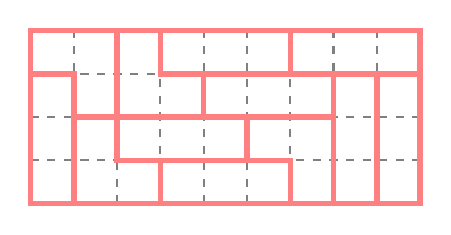
\begin{tikzpicture}[scale = 0.55]
  \draw[thick, dashed, gray] (1,1) grid (10,5);
  \draw[line width = 2, red!50]
    (2,1)--(2,4)--(1,4)--(1,1)--cycle--(4,1)--(4,2)--(3,2)--(3,3)--(2,3)
    (1,4)--(1,5)--(3,5)--(3,3)--(6,3)--(6,2)--(4,2)
    (4,1)--(7,1)--(7,2)--(6,2)
    (7,1)--(8,1)--(8,3)--(6,3)
    (8,1)--(9,1)--(9,4)--(8,4)--(8,3)
    (9,4)--(10,4)--(10,1)--(9,1)
    (10,4)--(10,5)--(7,5)--(7,4)--(8,4)
    (7,4)--(5,4)--(5,3)
    (5,4)--(4,4)--(4,5)--(3,5)
    (4,5)--(7,5)
  ;
\end{tikzpicture}